\documentclass[border=3pt]{standalone}
%\usepackage{amsthm}
\usepackage{amsmath}
\usepackage{amssymb}
\usepackage{natbib}
\usepackage[colorlinks,citecolor=blue,urlcolor=blue,filecolor=blue,backref=page]{hyperref}
\usepackage{graphicx}
\usepackage{subfigure}
\usepackage{bm}
\usepackage{booktabs}
\usepackage{listings}
\usepackage{color}

\usepackage{tikz}
\usetikzlibrary{shapes.misc}
\usetikzlibrary{matrix}
\usetikzlibrary{arrows,backgrounds,fit,calc,shapes,automata}
\usetikzlibrary{bayesnet}
\tikzstyle{every picture}+=[remember picture]
\tikzset{
    %Define standard arrow tip
    >=stealth',
    %Define style for boxes¡
    punkt/.style={
           rectangle,
           rounded corners,
           draw=black,
           thick,
           text width=3.5cm,
           minimum height=1.0cm,
           text centered},
    % Define arrow style
    pil/.style={
           ->,
           thick,
           shorten <=2pt,
           shorten >=2pt,}
}
\usetikzlibrary{decorations.pathreplacing,shapes}
\pagestyle{empty}

\begin{document}
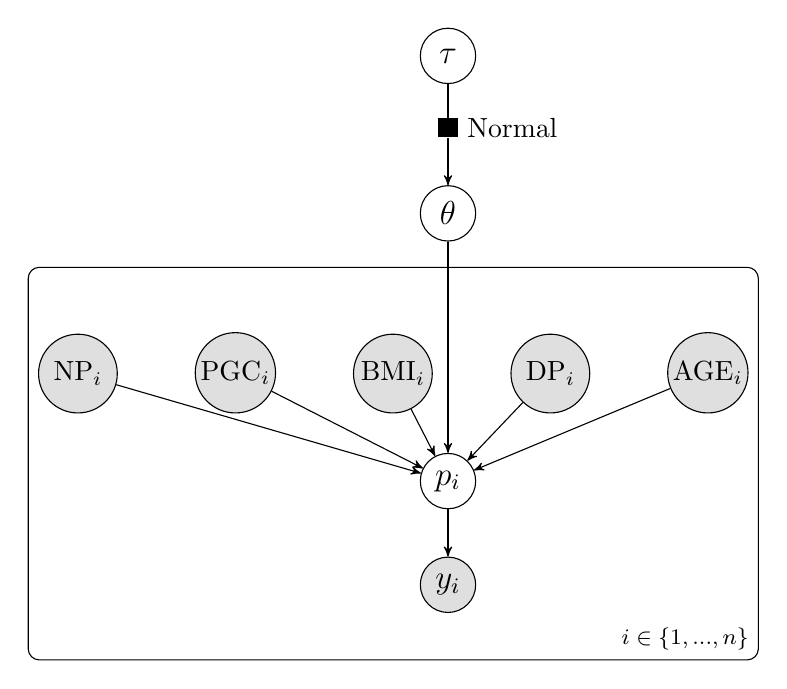
\begin{tikzpicture}[scale=1.0, transform shape]
  [squarednode/.style={rectangle, draw=black, minimum size=8mm},
    latent/.style={circle, draw=black, minimum size=10mm}]

  % \footnotesize

  % Define nodes
  \node[obs] (y) {\large $y_i$};
  \node[latent, above=6cm of y, xshift=0.0cm]  (tau) {\large $\tau$};
  \node[const, above=3.5cm of y] (dummy_top) {};

  % Theta --> P
  \node[latent, above=4cm of y, xshift=0.0cm]  (theta) {\large $\theta$};
  \node[factor, above=0.6cm of theta, xshift=0cm]  (N) {N};
  \node[const, right=0.1cm of N] () {\normalsize Normal};

  \node[latent, above=.6cm of y, xshift=0.0cm]  (P) {\large $p_{i}$};

  % Covariate 1 -->
  \node[obs, above=0.5cm of P, xshift=-4.7cm,  minimum size=1.0cm] (X1) {NP$_i$};

  % Covariate 2 -->
  \node[obs, above=0.5cm of P, xshift=-2.7cm,  minimum size=1.0cm] (X2) {PGC$_i$};

  % Covariate 3 -->
  \node[obs, above=0.5cm of P, xshift=-0.7cm, minimum size=1.0cm] (X3) {BMI$_i$};

  % Covariate 4 -->
  \node[obs, above=0.5cm of P, xshift=1.3cm, minimum size=1.0cm] (X4) {DP$_i$};

  % Covariate 5 -->
  \node[obs, above=0.5cm of P, xshift=3.3cm,  minimum size=1.0cm] (X5) {AGE$_i$};


  \draw [->] (P) -- (y);


  \draw [->] (X1) -- (P);
  \draw [->] (X2) -- (P);
  \draw [->] (X3) -- (P);
  \draw [->] (X4) -- (P);
  \draw [->] (X5) -- (P);

  \draw [->] (theta) -- (P);

  \factoredge{tau}{N}{theta}


  \plate {} {(dummy_top)(X1)(P)(X5)(y)} {$i \in \lbrace 1, ..., n \rbrace$}; %

\end{tikzpicture}
\end{document}
